\section[Vyhořívání]{Výpočty vyhoření jaderného paliva, formulace úlohy a metoda prediktor-korektor}

\subsection{Formulace úlohy}

Vyhoření se počítá jednogrupově pomocí modifikovaných Batemanových rovnic:

\begin{equation}
  \dfrac{\text{d}N_i}{\text{d}t} = -\sigma_i \: \phi N_i + \sum_{j \neq i} \left(\gamma_{j \to i} \: \sigma_{j \to i} \: \phi N_j \right) - \lambda_i N_i + \sum_{j \neq i} \left( \gamma_{j \to i} \: \lambda_{j \to i} \: N_j \right),
\end{equation}

kde $N_i$ představuje atomovou koncentraci $i$-tého nuklidu, $\phi \sigma_i$ představuje reakční rychlost na $i$-tém izotopu, $\lambda_i$ představuje rozpadovou konstantu $i$-tého izotopu a $\gamma$ představuje výtěžek dané reakce, resp. radiační výtěžek.

Rovnici je možné zapsat i v maticové podobě ve tvaru:

\begin{equation}
  \dfrac{\text{d}\vec{N}}{\text{d}t} = \mathbf{B} \cdot \vec{N},
\end{equation}

kde $\mathbf{B}$ představuje vyhořívající matici obsahující veškeré reakční rychlosti přechodů z $j$-tého izotopu na $i$-tý.

Samotná vyhořívající matice je velmi řídká a zpravidla se sestavuje tak, aby většina nenulových hodnot byla v okolí diagonály, případně do horního trojúhelníkového tvaru, což posléze zrychlí výpočet. V okolí diagonály se nacházejí reakce mezi atomy s podobnými hmotnostními čísly (radioaktivní rozpady, záchyty apod.), na pravé straně jsou produkty ze štěpení a v horní části produkty z reakcí (n,p), (n,t) apod. Jinými slovy, osa $x$ říká co vstupuje do reakce, osa $y$ co vystupuje a hodnota na průsečíku je daná reakční rychlost, tedy pravděpodobnost reakce, viz obrázek:

\begin{figure}[H]
  \centering
  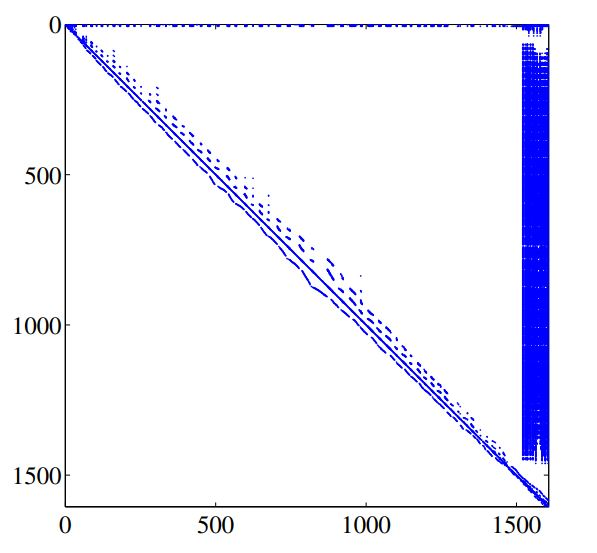
\includegraphics[width=0.5\textwidth]{img/burnup_matrix.JPG}
  \caption{Ukázka obsazenosti vyhořívající matice.}
\end{figure}

\subsection{Iterační schéma}

Obecně by šlo o jednoduché řešení, nicméně problémem je, že neznáme hodnotu $\phi$, která se stanovuje za pomoci normalizace výkonu. Problém je, že i kdyby byl výkon konstantní (což být nemusí), tak hustota toku neutronů v průběhu vyhoření konstantní nebude.

Nejjednodušším způsobem ke stanovení je uvažovat ji po celou dobu konstantní. Spočtu ji v daném čase a pak řeším soustavu LDR, což by stačilo vyřešit dopředným Eulerem. Toto zanedbání je aplikovatelné pouze pro malé časové kroky v ustáleném stavu, nebo pro výpočet složení vyhořelého paliva (kde je hustota toku nulová, teddy skutečně konstantní :) ).

Pro delší časové kroky (výpočet kampaně, ustalování při najetí, změny výkonu apod.) už to možné není. Problém je, že jak přibývají štěpné produkty, tak roste parazitní absorbce, což má za následek nutný nárůst hustoty toku. Ideální by tedy bylo pro vyhoření uvažovat střední hustotu toku neutronů v polovině kroku, nicméně tu neznám, jelikož neznám hustotu toku na konci kroku. Proto se postupuje pomocí tzv. metody \textbf{prediktor-korektor}, která nejprve odhadne $\phi$ na začátku cyklu, dopočte na konec cyklu (prediktor), přepočte novou $\phi$ z konce. Z těchto dvou hodnot poté stanoví průměr (korektor) a dopočte nové složení na konci cyklu.

Dále je možné rozlišit dva způsoby extrapolace prvotního odhadu prediktoru. V prvním kroku výpočtu se vždy musí určit za pomoci konstantní extrapolace, jelikož neznám předchozí průběh. Nicméně tím jak kroky přibývají, tak je možné pro další odhady uvažovat extrapolace vyšších řádů (v praxi asi jenom lineární), což prvotní odhad zpřesní. Druhý krok korektor je už vždy na základě lineární extrapolace mezi začátkem a koncem. Rozlišujeme tedy metody CONST/LIN a LIN/LIN.

Z tohoto důvodu je důležité vhodně stanovit délku kroku. Například u tepelných systémů je třeba počáteční kroky volit velmi krátké, jelikož dochází k ustalování koncentrace xenonu, což má za následek velký nárůst $\phi$. U rychlých systémů to tak kritické není.

Dále je potřebná nodalizace. Hustota toku se prostorově liší (jiná je ve středu vs. na kraji, dále větší štěpení na obvodu proutků kvůli samostínění). Palivo se tedy rozdělí do několika nódů a v každém nódu se řeší Batemanovy rovnice samostatně.

\subsection{Způsoby řešení}

Zmíněná schémata sloužila pouze na odhad hustoty toku. Stále máme kombinaci LDR o tisícech členů, což je značně nestabilní (knihovny jaderných dat mohou mít definované účinné průřezy pro stovky nuklidů a rozpadová data až pro tisíce nuklidů). Proto se musí úloha zjednodušit a uvažovat pouze některé z izotopů, např. ty, které se v daném transmutačním schématu skutečně mohou nacházet. V praxi se pak řeší řádově "pouze" nějakých 1500 nuklidů.

Když známe hustotu toku, je možné přejít k numerickému řešení.

\subsubsection{MATREX metoda}

Asi nejjednodušší metoda, která řeší přímo maticovou formu Batemanových rovnic:

\begin{equation}
  \dfrac{\text{d}\vec{N}}{\text{d}t} = \mathbf{B} \cdot \vec{N}(t)
\end{equation}

ve formě exponenciály:

\begin{equation}
  \vec{N}(t) = \text{exp} (\mathbf{B}t) \: \vec{N}(0).
\end{equation}

Exponenciální matici není možné přesně vyjádřit, proto se přechází ke zjednodušením. Pro MATREX metodu se exponenciála určí jako:

$$ \text{exp} (\mathbf{B}t) = \sum_{k=0}^\infty \dfrac{(\mathbf{B}t)^k}{k!}. $$

Je to takovej divnej dopřednej Euler pro maticový zápis LDR. 

\subsubsection{CRAM metoda}

Neboli aproximace pomocí Chebyshevových racionálních funkcí. Obyčejně se využívá CRAM metoda 16. řádu, která má stejnou přesnost, jenom je rychlejší než MATREX metoda.

Funguje na stejném základu, pouze rozkládá exponenciální matici do Chebyshevových racionálních funkcí:

$$ \vec{N}(t) = \left [ \sum_{k=0}^\infty \dfrac{(\textbf{A}t)^k}{k!} \right ] \vec{N}(0) \approx \left [ \alpha_{0,K} \textbf{I} + 2 \text{Re} \left [ \sum_{j=1}^{K/2} \left ( -\dfrac{\alpha_{j,K}}{\theta_{j,K}} \right ) \left ( \textbf{I} + \textbf{A} \left ( -\dfrac{t}{\theta_{j,K}} \right ) \right ) ^{-1} \right ] \right ] \vec{N}(0), $$

kde $K$ představuje řád a $\alpha_{i,j}$ a $\theta_{i,j}$ jsou příslušné CRAMerovy koeficienty k dohledání v literatuře.

\subsubsection{Analýza transmutační trajektorie}

Vychází z rozvoje jednotlivých transmutací a přeměn do lineárních řetězců. Vyjde se ze základního izotopu a na něj se postupně vrství jednotlivé trajektorie reakcí, co a jak může vzniknout, přičemž se uvažuje, že nenulová počáteční koncentrace je pouze pro zmíněný prvotní nuklid.

Začnu teda třeba $^{238}$U, z něj zjistím že se může transmutovat na $^{239}$U, ten se může transmutovat na $^{240}$U nebo přeměnit na $^{239}$Np apod. Problém je, že situace v reaktoru je natolik komplikovaná a provázaná, že není možné podchytit všechny reakce a dochází ke zjednodušování řetězců a k upřednostňování jenom vybraných dle důležitosti, případně k ukončení řetězce, pokud dojde k poklesu koncentrace pod stanovenou hodnotu.

Další problém je, že může docházet ke smyčkám, např. $^{235}$U přes nepružný rozptyl (n,2n) na $^{234}$U a ten přes záchyt zpět na $^{235}$U. To se řeší za pomoci zavedení drobných odchylek do řetězce do opakujících se konstant (což jsou ty účinné průřezy), které jsou ovšem pod mezí neurčitosti a za pomoci kterých nekonečné smyčky po chvíli vymizí.